% Created 2021-10-27 mié 18:30
% Intended LaTeX compiler: pdflatex
\documentclass[11pt]{article}
\usepackage[utf8]{inputenc}
\usepackage[T1]{fontenc}
\usepackage{graphicx}
\usepackage{grffile}
\usepackage{longtable}
\usepackage{wrapfig}
\usepackage{rotating}
\usepackage[normalem]{ulem}
\usepackage{amsmath}
\usepackage{textcomp}
\usepackage{amssymb}
\usepackage{capt-of}
\usepackage{hyperref}
\usepackage{fullpage}
\usepackage{indentfirst}
\author{Martín Rossi}
\date{}
\title{Trábajo práctico IPv6}
\hypersetup{
 pdfauthor={Martín Rossi},
 pdftitle={Trábajo práctico IPv6},
 pdfkeywords={},
 pdfsubject={},
 pdfcreator={Emacs 27.2 (Org mode 9.4.4)}, 
 pdflang={English}}
\begin{document}

\maketitle
\section*{1. Wireshark}
\label{sec:orgae3beb9}
\subsection*{1.c.}
\label{sec:org7ef75ed}
\begin{center}
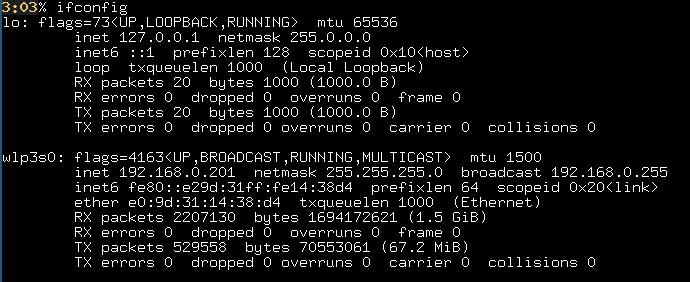
\includegraphics[width=.9\linewidth]{./1c.png}
\end{center}

Primero se ve la interfaz loopback (lo) con direcciones 127.0.0.1 y ::1 para IPv4 e IPv6.

Después se ve otra interfaz wlp3s0, que tiene dirección IPv6 fe80::e29d:31ff:fe14:38d4 con el prefijo fe80 que indica una dirección link local, o sea que es válida sólo para el enlace local. Su dirección MAC es e0:9d:31:14:38:d4.
\subsection*{1.d.}
\label{sec:orgf538e9d}
\begin{center}
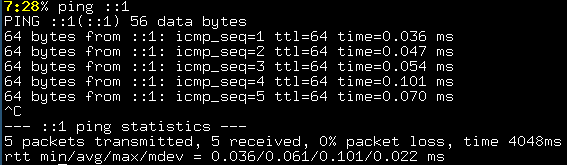
\includegraphics[width=.9\linewidth]{./1d.png}
\end{center}
\newpage
\subsection*{1.e.}
\label{sec:org29aa312}
No pude hacer este ejercicio con IPv6, así que usé direcciones IPv4 para ver los paquetes capturados.
\begin{center}
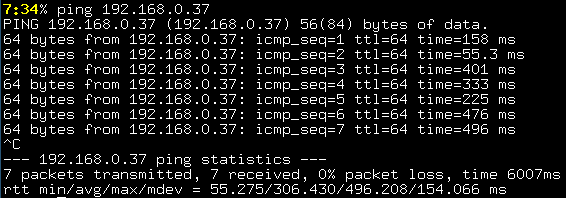
\includegraphics[width=.9\linewidth]{./1ea.png}
\end{center}
\begin{center}
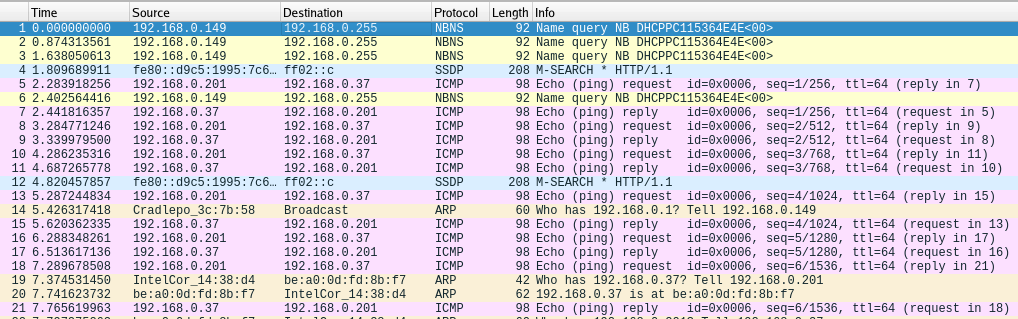
\includegraphics[width=.9\linewidth]{./1eb.png}
\end{center}

Se pueden ver los paquetes ICMP en rojo de los ping request y reply entre 192.168.0.37 y 192.168.0.201. La información adicional que se muestra es el id del mensaje ping, el número de secuencia y el time to live (ttl).
\subsection*{1.f.}
\label{sec:org32d59f4}
\begin{center}
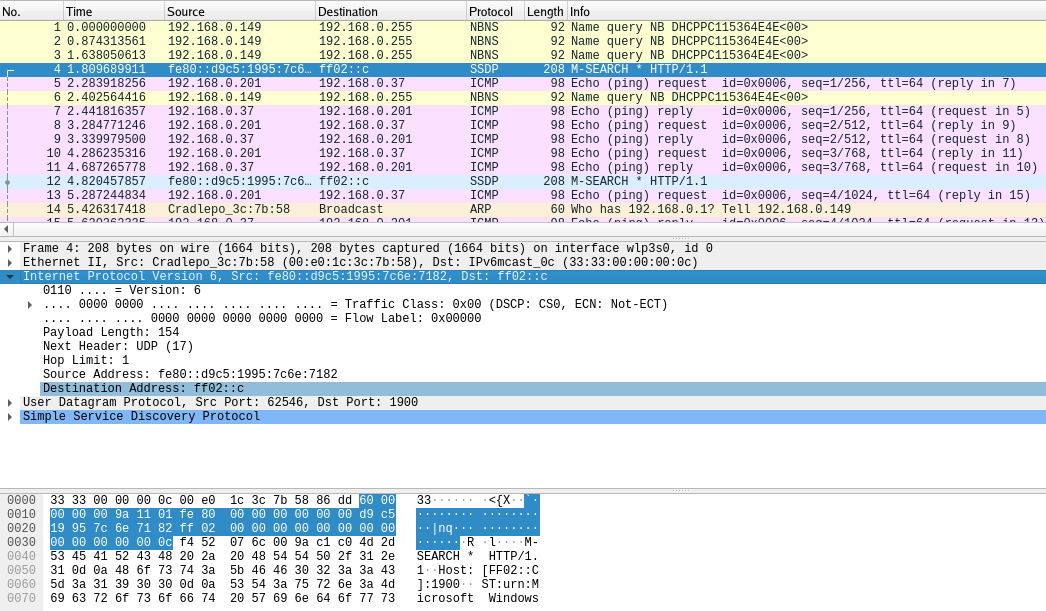
\includegraphics[width=.9\linewidth]{./1f.png}
\end{center}
Se puede ver que la cabecera del paquete tiene los campos:
\begin{itemize}
\item versión: 0110 (6)
\item trafic class: 0x00
\item flow label: 0x00000
\item payload length: 154
\item next header: 17 (UDP)
\item hop limit: 1
\item source address
\item destination address
\end{itemize}
\newpage
\subsection*{1.g.}
\label{sec:org3745e57}
\begin{center}
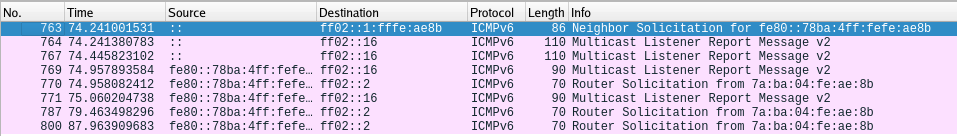
\includegraphics[width=.9\linewidth]{./1g.png}
\end{center}

Cuando se conectó un nodo nuevo pude capturar los siguientes paquetes ICMPv6:
\begin{itemize}
\item \textbf{Neighbor Solicitation:} tipo 135. Se usa para determinar direcciones MAC de los vecinos.
\end{itemize}
\begin{center}
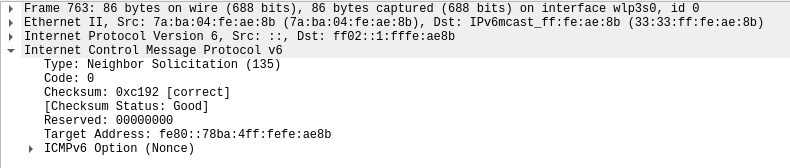
\includegraphics[width=.9\linewidth]{./1ga.png}
\end{center}
\begin{itemize}
\item \textbf{Multicast Listener Report Message:} tipo 143. Es para descubrir nodos que deseen recibir paquetes multicast.
\end{itemize}
\begin{center}
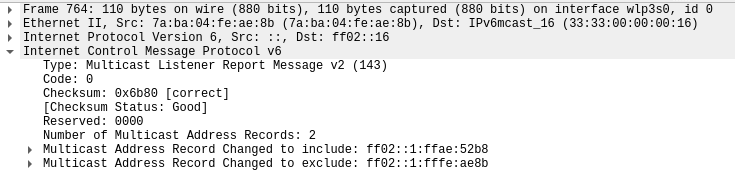
\includegraphics[width=.9\linewidth]{./1gb.png}
\end{center}
\begin{itemize}
\item \textbf{Router Solicitation:} tipo 133. Cuando un nodo nuevo se conecta pide al router que se anuncie para informar a los nodos.
\end{itemize}
\begin{center}
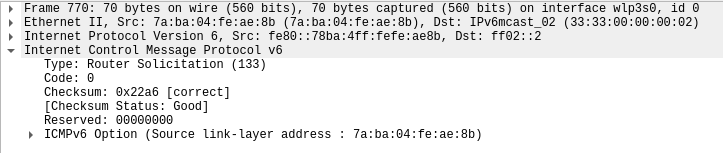
\includegraphics[width=.9\linewidth]{./1gc.png}
\end{center}
\newpage
\section*{2. Packet tracer}
\label{sec:org7801212}
\subsection*{Tarea 2.}
\label{sec:orgce3fb4d}
\subsubsection*{b.}
\label{sec:org9de6d34}
Las 4 interfaces tienen IPv6 habilitado.
\begin{center}
\begin{tabular}{llll}
\textbf{Dispositivo} &  & \textbf{Dirección IP local} & \textbf{Dirección IP global}\\
\hline
\textbf{Router0} & \textbf{Fa0/0} & FE80::202:4AFF:FE35:6301 & 2001:DB8:1:0:202:4AFF:FE35:6301\\
 & \textbf{Fa0/1} & FE80::202:4AFF:FE35:6302 & 2001:DB8:2:0:202:4AFF:FE35:6302\\
\hline
\textbf{Router1} & \textbf{Fa0/0} & FE80::2D0:BCFF:FE88:ED01 & 2001:DB8:3:0:2D0:BCFF:FE88:ED01\\
 & \textbf{Fa0/1} & FE80::2D0:BCFF:FE88:ED02 & 2001:DB8:2:0:2D0:BCFF:FE88:ED02\\
\end{tabular}
\end{center}

Router0:
\begin{center}
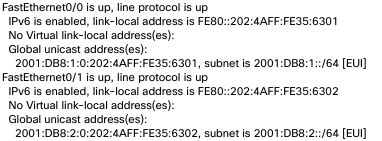
\includegraphics[width=.9\linewidth]{./router0.png}
\end{center}

Router1:
\begin{center}
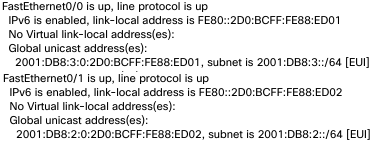
\includegraphics[width=.9\linewidth]{./router1.png}
\end{center}
\newpage
\begin{enumerate}
\item Una dirección IPv6 tiene 128 bits.
\item El prefijo es 2001:DB8:1::/64 y el ID de la interface es 202:4AFF:FE35:6301.
\item La MAC es 0002.4A35.6301. El ID de la interface se forma dividiendo la MAC en dos partes de 24 bits, agregando en el medio FFFE e invirtiendo el séptimo bit, por lo que el primer grupo pasa de 0002 a 0202. Éste es el formato EUI-64.
\end{enumerate}
\subsubsection*{c.}
\label{sec:orgc5de811}
Router0:
\begin{center}
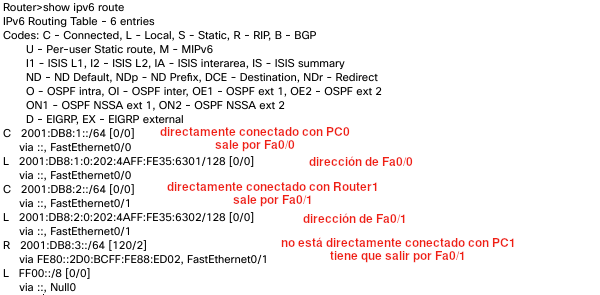
\includegraphics[width=.9\linewidth]{./r0route.png}
\end{center}

Router1:
\begin{center}
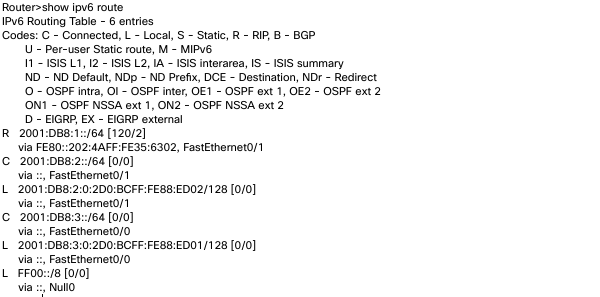
\includegraphics[width=.9\linewidth]{./r1route.png}
\end{center}
\subsubsection*{d.}
\label{sec:org5a96f7c}
\begin{center}
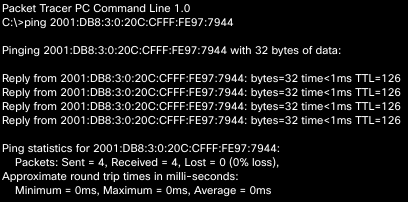
\includegraphics[width=.9\linewidth]{./ping.png}
\end{center}
\subsection*{Tarea 3.}
\label{sec:orgea86017}
\begin{center}
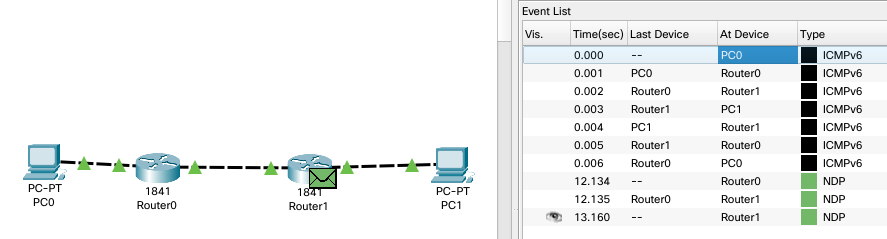
\includegraphics[width=.9\linewidth]{./icmp.png}
\end{center}
\begin{itemize}
\item PC0 crea el paquete ICMPv6 y lo manda a la puerta de enlace predeterminada, que es Router0.
\item Router0 recibe el paquete, se fija el destino y mira en la tabla de ruteo para dónde tiene que dirigirlo. La tabla indica que tiene que enviarlo por el enlace a Router1.
\item Router1 hace lo mismo, pero en este caso ve que el destino está directamente conectado. Lo envía por el enlace correspondiente.
\item PC1 recibe el paquete y prepara la respuesta.
\item Se da el proceso inverso.
\item Sigue con paquetes NDP de router advertisement.
\end{itemize}
\newpage
\subsection*{Tarea 4.}
\label{sec:org0bacb53}
\subsubsection*{d.}
\label{sec:orgd1ef21c}
Paquetes ICMPv6 que se envían desde PC0 con tipo 128 \emph{echo request}, y los que devuelve PC1 con tipo 129 de \emph{echo reply}. Las direcciones IP de origen y destino se mantienen, lo que cambia son las direcciones MAC de las tramas que son de los dos routers intermedios.
\begin{center}
\begin{tabular}{ll}
\hline
\textbf{Tipo} & 128\\
\textbf{Dirección Fuente} & 2001:db8:1:0:201:96ff:fe1d:8173 (PC0), 0001.961d.8173 (MAC Fa0 PC0)\\
\textbf{Dirección Destino} & 2001:db8:3:0:20c:cfff:fe97:7944 (PC1), 0002.4a35.6301 (MAC Fa0/0 Router0)\\
\textbf{Dato} & \\
\hline
\textbf{Tipo} & 128\\
\textbf{Dirección Fuente} & 2001:db8:1:0:201:96ff:fe1d:8173 (PC0), 0002.4a35.6302 (MAC Fa0/1 Router0)\\
\textbf{Dirección Destino} & 2001:db8:3:0:20c:cfff:fe97:7944 (PC1), 00d0.bc88.ed02 (MAC Fa0/1 Router1)\\
\textbf{Dato} & \\
\hline
\textbf{Tipo} & 128\\
\textbf{Dirección Fuente} & 2001:db8:1:0:201:96ff:fe1d:8173 (PC0), 00d0.bc88.ed01 (MAC Fa0/0 Router1)\\
\textbf{Dirección Destino} & 2001:db8:3:0:20c:cfff:fe97:7944 (PC1), 000c.cf97.7944 (MAC Fa0 PC1)\\
\textbf{Dato} & \\
\hline
\textbf{Tipo} & 129\\
\textbf{Dirección Fuente} & 2001:db8:3:0:20c:cfff:fe97:7944 (PC1), 000c.cf97.7944 (MAC Fa0 PC1)\\
\textbf{Dirección Destino} & 2001:db8:1:0:201:96ff:fe1d:8173 (PC0), 00d0.bc88.ed01 (MAC Fa0/0 Router1)\\
\textbf{Dato} & \\
\hline
\textbf{Tipo} & 129\\
\textbf{Dirección Fuente} & 2001:db8:3:0:20c:cfff:fe97:7944 (PC1), 00d0.bc88.ed02 (MAC Fa0/1 Router1)\\
\textbf{Dirección Destino} & 2001:db8:1:0:201:96ff:fe1d:8173 (PC0), 0002.4a35.6302 (MAC Fa0/1 Router0)\\
\textbf{Dato} & \\
\hline
\textbf{Tipo} & 129\\
\textbf{Dirección Fuente} & 2001:db8:3:0:20c:cfff:fe97:7944 (PC1), 0002.4a35.6301 (MAC Fa0/0 Router0)\\
\textbf{Dirección Destino} & 2001:db8:1:0:201:96ff:fe1d:8173 (PC0), 0001.961d.8173 (MAC Fa0 PC0)\\
\textbf{Dato} & \\
\hline
\end{tabular}
\end{center}
\newpage
\subsubsection*{e.}
\label{sec:org21e519d}
Estos son los paquetes que se envían desde que pongo configuración automática de IPv6 en PC0 hasta que aparece \emph{ipv6 request successful}
\begin{center}
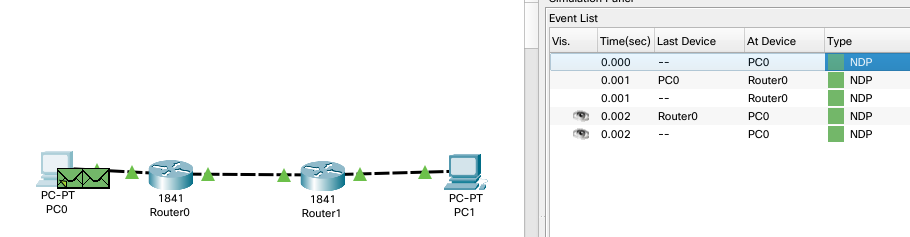
\includegraphics[width=.9\linewidth]{./4f.png}
\end{center}
\begin{center}
\begin{tabular}{ll}
\hline
\textbf{Tipo} & 133 (Router Solicitation Message)\\
\textbf{Dirección Fuente} & fe80::201:96ff:fe1d:8173 (PC0), 0001.961d.8173 (MAC Fa0 PC0)\\
\textbf{Dirección Destino} & ff02::2 (multicast local all routers)\\
\textbf{Dato} & \\
\hline
\textbf{Tipo} & 134 (Router Advertisement Message)\\
\textbf{Dirección Fuente} & fe80::202:4aff:fe35:6301 (Fa0/0 Router0), 0002.4a35.6301\\
\textbf{Dirección Destino} & ff02::1 (multicast local all nodes)\\
\textbf{Dato} & \\
\hline
\textbf{Tipo} & 135 (Neighbor Message)\\
\textbf{Dirección Fuente} & 2001:db8:1:0:201:96ff:fe1d:8173 (PC0), 0001.961d.8173 (MAC Fa0 PC0)\\
\textbf{Dirección Destino} & ff02::1:ff1d:8173\\
\textbf{Dato} & \\
\hline
\end{tabular}
\end{center}
\end{document}